\documentclass[aspectratio=169]{beamer}


\mode<presentation>
{
	\usetheme{Montpellier}
	\usecolortheme{whale}
	\usefonttheme{default}
	\setbeamertemplate{navigation symbols}{}
	\setbeamertemplate{caption}[numbered]
}

%enumerate continuing numbering
\setbeamercovered{highly dynamic}

\newcounter{saveenumi}
\newcommand{\seti}{\setcounter{saveenumi}{\value{enumi}}}
\newcommand{\conti}{\setcounter{enumi}{\value{saveenumi}}}
%

\usepackage[portuguese]{babel}
\usepackage[utf8x]{inputenc}
\usepackage[T1]{fontenc}
\usepackage{natbib}
\usepackage{hyperref}
\usepackage{enumerate}
\usepackage{subfig}
%\usepackage{biblatex}

%numbering
\addtobeamertemplate{navigation symbols}{}{%
	\usebeamerfont{footline}%
	\usebeamercolor[fg]{footline}%
	\hspace{1em}%
	\insertframenumber/\inserttotalframenumber
}

\title[Proposta de tese para o exame de qualificação]{Aprimoramentos em modelagem geológica implícita com funções distância assinaladas}
%\subtitle{Proposta de tese para o exame de qualificação}
\author{Me. Roberto Mentzingen Rolo \\ \small{Orientador: Prof. Dr. João Felipe Coimbra Leite Costa, PhD}}
\institute{Universidade Federal do Rio Grande do Sul \\ Escola de Engenharia \\ Programa de Pós-Graduação em Engenharia de Minas, Metalúrgica e de Materiais}
\date{17 de junho de 2019}

\begin{document}
	
%\section{Apresentação}
	
\begin{frame}
	\titlepage
\end{frame}

%sumário
\begin{frame}{Estrutura}
\begin{scriptsize}
	\tableofcontents
\end{scriptsize}
\end{frame}

\section{Introdução}

\begin{frame}{Introdução}

Construir modelos numéricos de longo, médio e curto prazo para avaliação de recursos/reservas e planejamento de mina exige quatro grandes atividades:

\begin{enumerate}
\item Coleta e gerenciamento de dados;
\item Interpretação e modelagem geológica;
\item Atribuição de teores;
\item Avaliação e gerenciamento da incerteza geológica e de teores.
\end{enumerate}

\end{frame}

\subsection{Interpretação e modelagem geológica}

\begin{frame}{Interpretação e modelagem geológica}

\begin{enumerate}
	\item Identificar diferentes domínios;
	\item Definir os limites de cada função aleatória estacionária.
\end{enumerate}

\begin{figure}[H]
	\begin{center}
		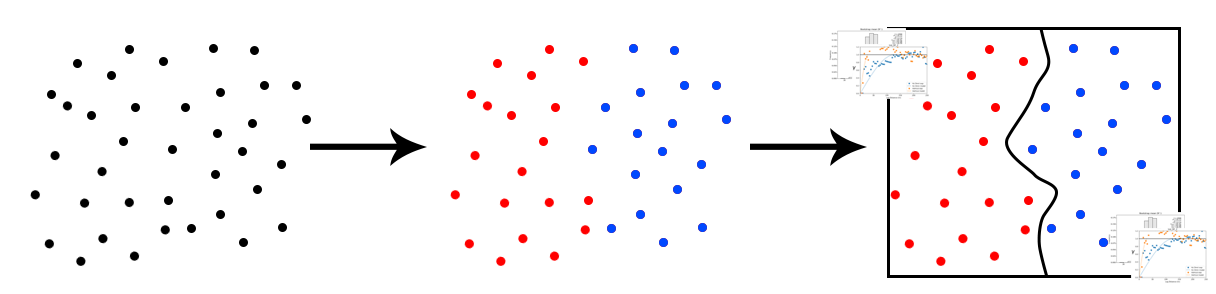
\includegraphics[width=\textwidth]{apresentacao/passo_2}
		\caption{Interpretação e modelagem geológica.}
	\end{center}
\end{figure}

\end{frame}

\subsection{Método tradicional}

\begin{frame}{Metodologia tradicional}

A abordagem tradicional para a criação de modelos geológicos tridimensionais é através da triangulação de polilinhas.

\begin{figure}[H]
	\begin{center}
		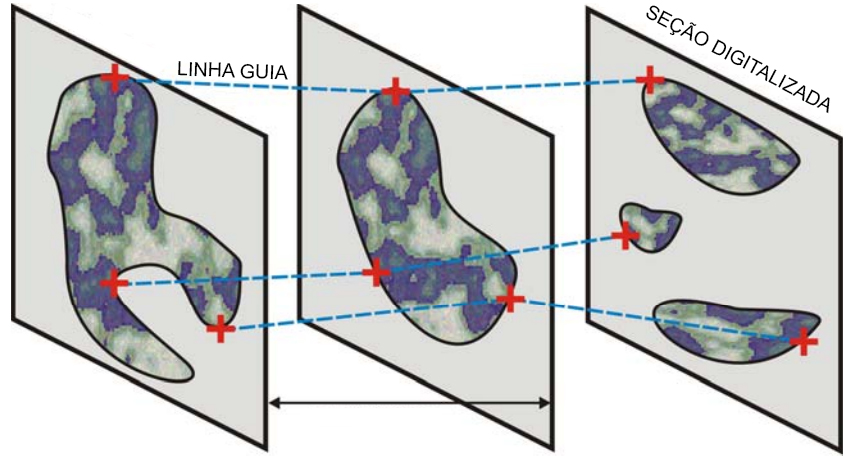
\includegraphics[width=0.6\textwidth]{capitulo_1/explicitmodeling}
		\caption{Esquema do método tradicional.}
	\end{center}
\end{figure}

\end{frame}

\begin{frame}{Desvantagens do método tradicional}
	\begin{itemize}
		\item Tedioso e demorado;
		\item Exige um profissional especializado e experiente;
		\item Geometria dos corpos precisa ser simplificada;
		\item Subjetivo;
		\item Não replicável;
		\item Inflexível;
		\item Não avalia a incerteza.
	\end{itemize}
\end{frame}

\subsection{Incerteza do modelo geológico}

\begin{frame}{Incerteza do modelo geológico}

Em muitos casos, a incerteza do modelo geológico pode ser uma fonte de incerteza crucial e deve ser avaliada.

\begin{figure}[H]
	\begin{center}
		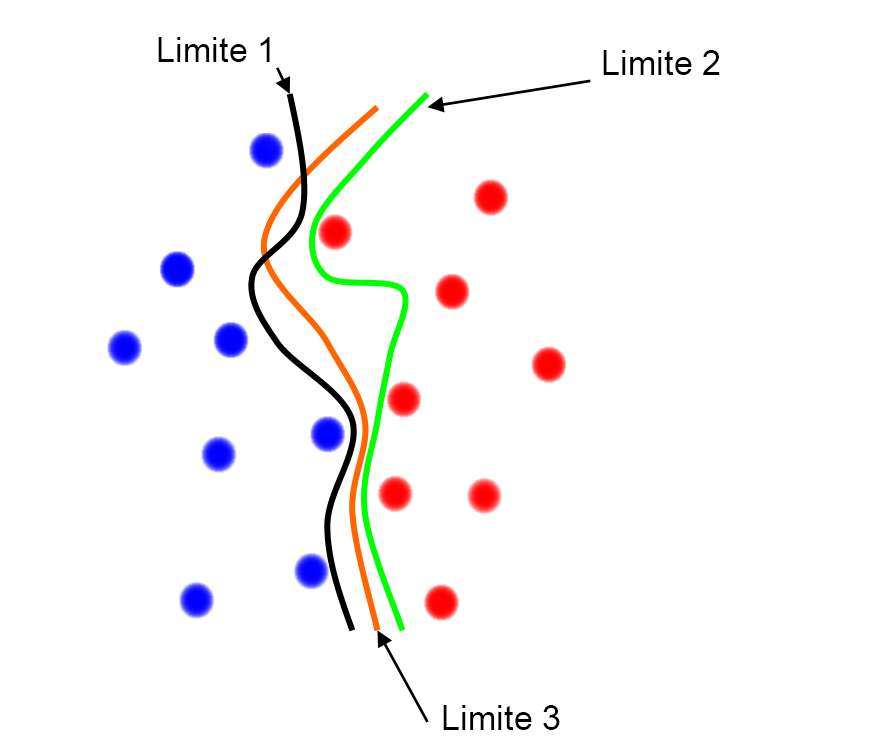
\includegraphics[width=0.4\textwidth]{capitulo_1/incerteza_limites}
		\caption{Incerteza do modelo geológico.}
	\end{center}
\end{figure}
\end{frame}

\subsection{Métodos matemáticos}

\begin{frame}{Métodos matemáticos}

	\begin{columns}[t]
		\begin{column}{0.5\textwidth}
			\begin{center}
				\textit{Métodos determinísticos}
			\end{center}
			\begin{itemize}
				\item Vizinho mais próximo;
				\item Krigagem dos indicadores.
			\end{itemize}
		\end{column}
		\begin{column}{0.5\textwidth}
			\begin{center}
				\textit{Métodos estocásticos}
			\end{center}
			\begin{itemize}
				\item Simulação sequencial dos indicadores;
				\item Simulação gaussiana/plurigaussiana truncada;
				\item Simulação multi ponto;
				\item Simulação baseada em objetos;
			\end{itemize}
		\end{column}
	\end{columns}
	
\end{frame}

\subsection{Métodos implícitos}

\begin{frame}{Métodos implícitos}
	\begin{figure}[H]
		\begin{center}
			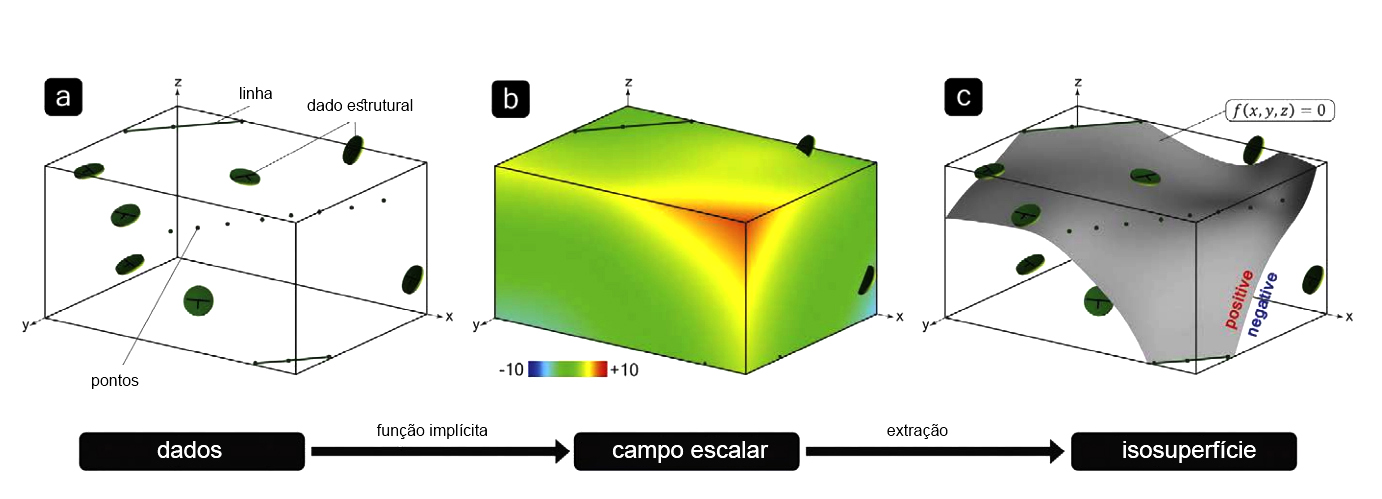
\includegraphics[width=0.8\textwidth]{capitulo_1/implicit_modelig_pt_1}
			\caption{Esquema dos métodos implícitos.}
		\end{center}
	\end{figure}
\end{frame}

\section{Modelagem geológica implícita com funções distância assinaladas}

\begin{frame}{O banco de dados}

72 furos totalizando 3349 amostras distribuídas entre 3 diferentes categorias.

	\begin{figure}
		\centering
		\subfloat[Proporções.]{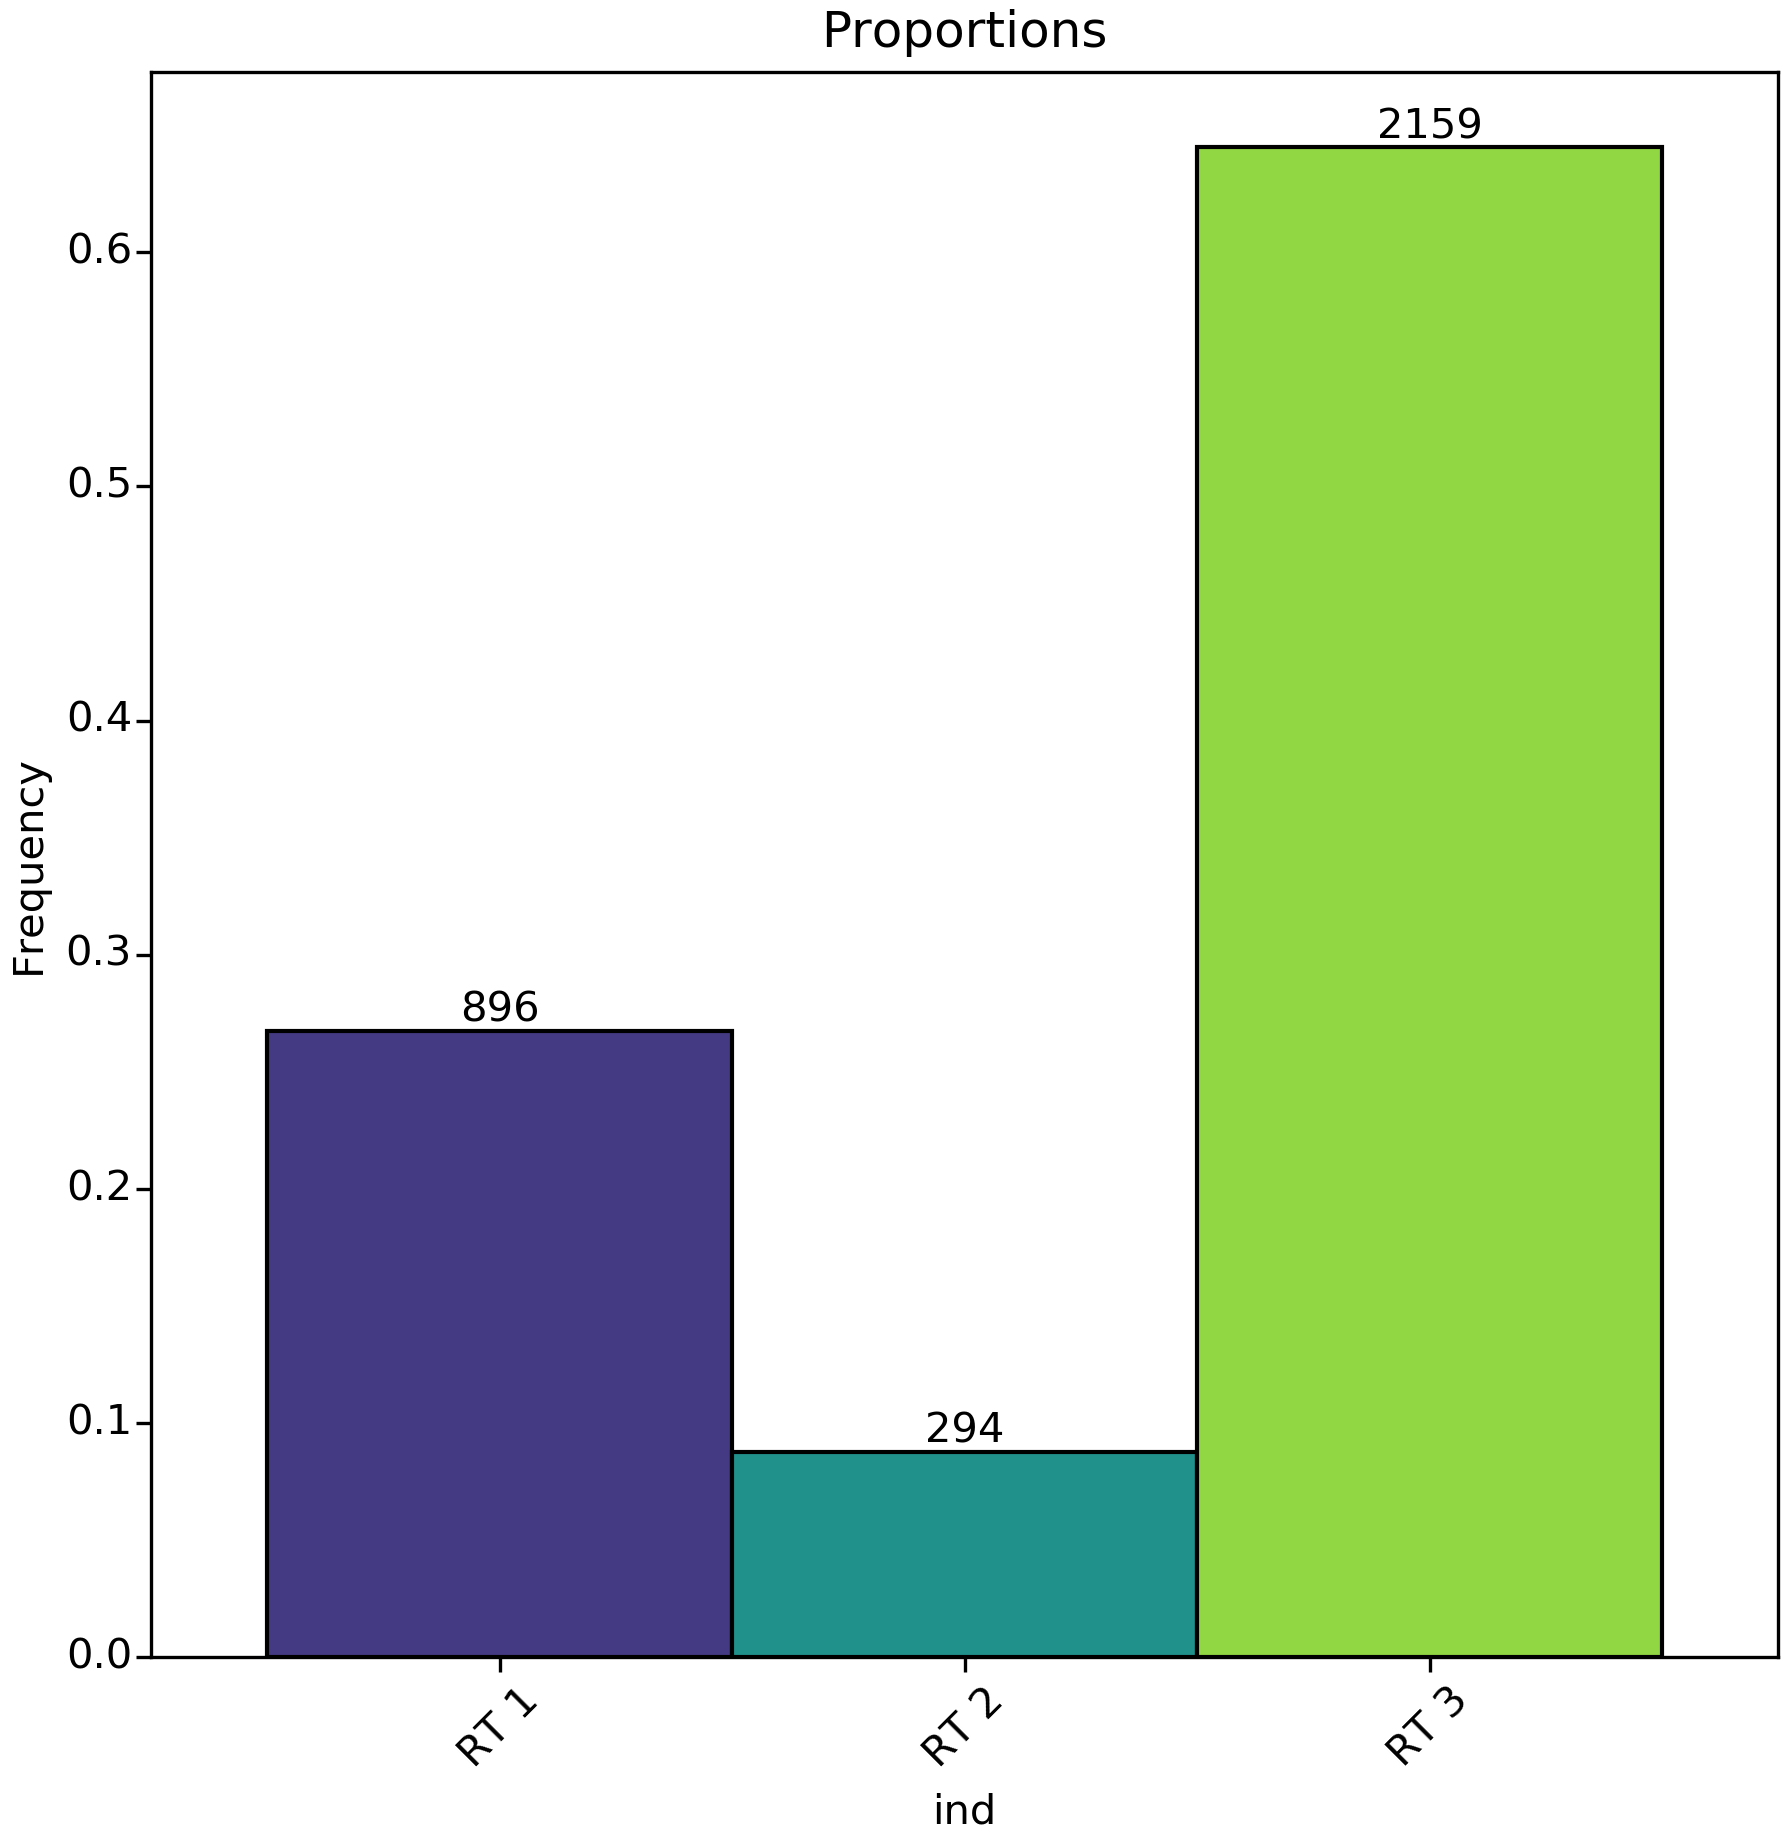
\includegraphics[width=.25\textwidth]{capitulo_2/prop_hist_big.png}}\hspace{20mm}
		\subfloat[Vista das amostras.]{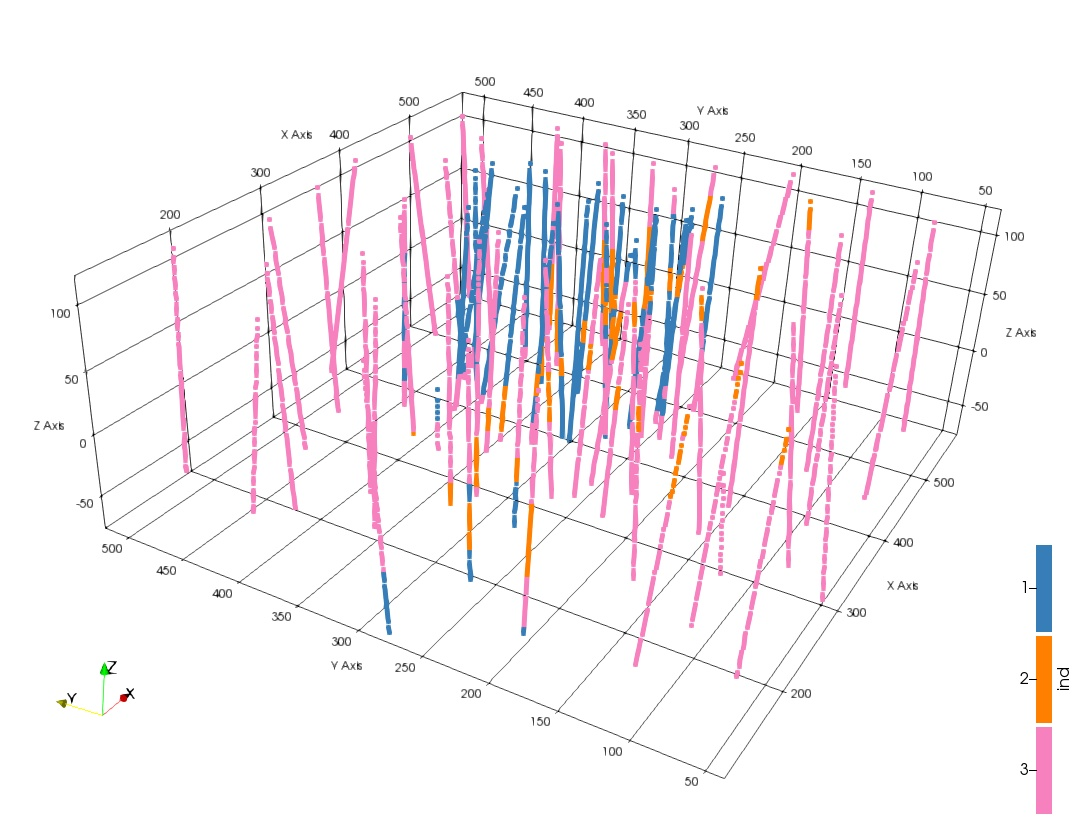
\includegraphics[width=.4\textwidth]{capitulo_2/dados.jpeg}}
		\caption{O banco de dados.}
	\end{figure}
		
\end{frame}

\end{document}